Multiple choice section. All points are for choosing the correct answer. No justification is needed.
\begin{questions} 

%\question[] MC
%\begin{choices}
%    \choice \chooseone
%    \choice \chooseone
%    \choice \chooseone
%    \choice \chooseone
%    \choice \chooseone None of the above.
%\end{choices}


\question[3] What is the domain for the function $g(x)=\dfrac{\sqrt{x+4}}{x}$?
\begin{choices}
    \choice \chooseone $[-4,\infty)$
    \choice \chooseone $[4,\infty)$
    \choice \chooseone $[-4,0)\bigcup (0,\infty)$
    \choice \chooseone $(0,\infty)$
    \choice \chooseone None of the above.
\end{choices}


\question[3] Let $f(t)=e^{2t}$ and $g(t)=\sqrt{t^2-1}$. What is $g\circ f(t)$? 
    \begin{choices}
   \choice \chooseone $g\circ f(t)=\sqrt{t^2-1}\cdot e^{2t}$
   \choice \chooseone $g\circ f(t)= e^{2\sqrt{t^2-1}}$
   \choice \chooseone $g\circ f(t)=\sqrt{e^{2(t^2-1)}}$
   \choice \chooseone $g\circ f(t)=\sqrt{(e^{2t})^2-1}$
   \choice \chooseone None of the above.
\end{choices}



\question %Polynomial graph
\begin{parts}
    \part[3] Find the end behavior of the polynomial $f(x)=x(x-3)^2$.
     \begin{choices}
    \choice \chooseone As $x\rightarrow -\infty$,  $f(x)\rightarrow+\infty$ and as
                            $x\rightarrow +\infty$, $f(x)\rightarrow +\infty$
    \choice \chooseone As $x\rightarrow -\infty$,  $f(x)\rightarrow-\infty$ and as
                            $x\rightarrow +\infty$, $f(x)\rightarrow -\infty$
        \choice \chooseone As $x\rightarrow -\infty$,  $f(x)\rightarrow-\infty$ and as
                            $x\rightarrow +\infty$, $f(x)\rightarrow +\infty$
    \choice \chooseone As $x\rightarrow -\infty$,  $f(x)\rightarrow+\infty$ and as 
                            $x\rightarrow +\infty$, $f(x)\rightarrow -\infty$
    \choice \chooseone None of the above.
     \end{choices}
    

    \part[3] Select the graph of $f(x)=x(x-3)^2$.
    
    \begin{multicols}{2}
    	
    	
    	\begin{choices}
    		\choice \chooseone\vspace{-.7cm}
    		
    		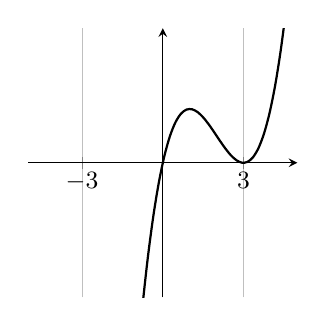
\begin{tikzpicture}%[domain=-4:4]
    			\begin{axis}[
    				grid=major,
    				axis x line = middle,
    				axis y line = middle,
    				%yticklabel style = {font=\tiny,xshift=0.5ex},
    				xticklabel style = {font=\small,yshift=0.5ex},
    				%scale only axis=true,
    				width=5 cm,
    				height=5 cm,
    				xtick={-3,0,3},%{-2,-1,0,1,2},
    				ytick=false,%{-2,-1,0,1,2,3,4},
    				xmin=-5,
    				xmax=5,
    				ymin=-10,
    				ymax=10,
    				]
    				%\draw[very thin,color=gray] (-2.9,-2.1) grid (2.9,2.9);
    				\addplot[smooth, thick, domain = -2:5,samples=35] { x*(x-3)^2};
    				%\addplot[smooth, thick, domain = 0:3,samples=35] { -x};
    			\end{axis}
    		\end{tikzpicture}
    		
    		\choice \chooseone\vspace{-.7cm}
    		
    		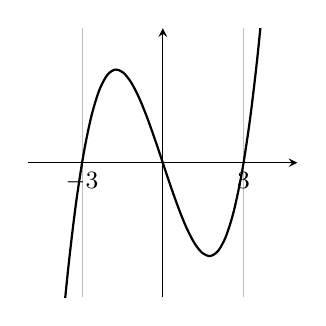
\begin{tikzpicture}%[domain=-4:4]
	\begin{axis}[
		grid=major,
		axis x line = middle,
		axis y line = middle,
		%yticklabel style = {font=\tiny,xshift=0.5ex},
		xticklabel style = {font=\small,yshift=0.5ex},
		%scale only axis=true,
		width=5 cm,
		height=5 cm,
		xtick={-3,0,3},%{-2,-1,0,1,2},
		ytick=false,%{-2,-1,0,1,2,3,4},
		xmin=-5,
		xmax=5,
		ymin=-15,
		ymax=15,
		]
		%\draw[very thin,color=gray] (-2.9,-2.1) grid (2.9,2.9);
		\addplot[smooth, thick, domain = -5:5,samples=35] { x*(x-3)*(x+3)};
		%\addplot[smooth, thick, domain = 0:3,samples=35] { -x};
	\end{axis}
\end{tikzpicture}
    		\\
    		\choice \chooseone\vspace{-.7cm}
    		
    		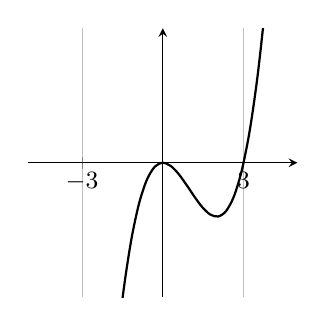
\begin{tikzpicture}%[domain=-4:4]
	\begin{axis}[
		grid=major,
		axis x line = middle,
		axis y line = middle,
		%yticklabel style = {font=\tiny,xshift=0.5ex},
		xticklabel style = {font=\small,yshift=0.5ex},
		%scale only axis=true,
		width=5 cm,
		height=5 cm,
		xtick={-3,0,3},%{-2,-1,0,1,2},
		ytick=false,%{-2,-1,0,1,2,3,4},
		xmin=-5,
		xmax=5,
		ymin=-10,
		ymax=10,
		]
		%\draw[very thin,color=gray] (-2.9,-2.1) grid (2.9,2.9);
		\addplot[smooth, thick, domain = -5:5,samples=35] { x^2*(x-3)};
		%\addplot[smooth, thick, domain = 0:3,samples=35] { -x};
	\end{axis}
\end{tikzpicture}
    		\choice \chooseone\vspace{-.7cm}
    		
    		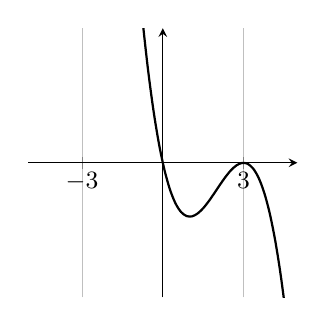
\begin{tikzpicture}%[domain=-4:4]
	\begin{axis}[
		grid=major,
		axis x line = middle,
		axis y line = middle,
		%yticklabel style = {font=\tiny,xshift=0.5ex},
		xticklabel style = {font=\small,yshift=0.5ex},
		%scale only axis=true,
		width=5 cm,
		height=5 cm,
		xtick={-3,0,3},%{-2,-1,0,1,2},
		ytick=false,%{-2,-1,0,1,2,3,4},
		xmin=-5,
		xmax=5,
		ymin=-10,
		ymax=10,
		]
		%\draw[very thin,color=gray] (-2.9,-2.1) grid (2.9,2.9);
		\addplot[smooth, thick, domain = -2:5,samples=35] { -x*(x-3)^2};
		%\addplot[smooth, thick, domain = 0:3,samples=35] { -x};
	\end{axis}
\end{tikzpicture}

      \choice \chooseone None of the above.
    	\end{choices}
    \end{multicols}
\end{parts}
\newpage

\question[3] The line parallel to $y=-3x+2$ through the point $(1,4)$ is given by:
\begin{choices}
    \choice \chooseone $y=3(x-1)+4$
    \choice \chooseone $y=-3(x-1)+4$
    \choice \chooseone $y=-3(x+1)-4$
    \choice \chooseone $y=\frac{1}{3}(x-1)+4$
    \choice \chooseone None of the above.
\end{choices}

\question[3] %2.3-2.4, graphing/functions
Choose the function represented by the graph, $y = f(x)$, below. 
\begin{center}
	
	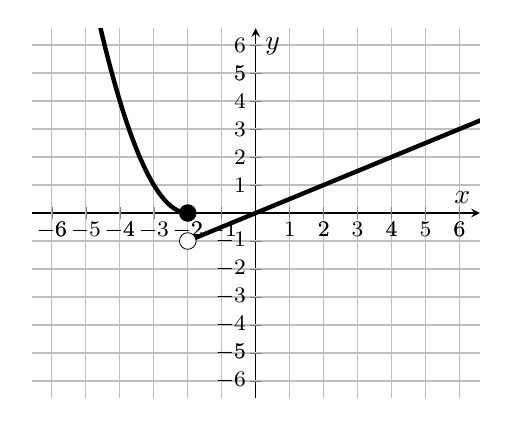
\begin{tikzpicture}
		\begin{axis}[
			grid = major,
			extra x ticks={-6,-5,-4,-3,-2,-1,1,2,3,4,5,6},
			extra y ticks={-6,-5,-4,-3,-2,-1,1,2,3,4,5,6},
			%xminorgrids=true,
			width=.6\textwidth,
			%clip = true,
			%clip mode=individual,
			%restrict y to domain=-12:12,
			axis x line = middle,
			axis y line = middle,
			yticklabel style = {font=\footnotesize,xshift=0.5ex},
			xticklabel style = {font=\footnotesize,yshift=0.5ex},
			xlabel={$x$},
			%xlabel style={at=(current axis.right of origin)},
			ylabel={$y$},
			%ylabel style={at=(current axis.above origin)},
			%domain = -5:5,
			xmin = -6,
			xmax = 6,
			enlarge y limits={rel=0.05},
			enlarge x limits={rel=0.05},
			ymin = -6,
			ymax = 6,
			]
			\addplot [smooth, ultra thick,
			domain=-6:-2, 
			samples=25, 
			color=black,
			]
			{(x+2)^2};
			
			% \addplot [smooth, ultra thick,
			% domain=-1:2, 
			% samples=25, 
			% color=black,
			% ]
			% {-x};
			
			\addplot [smooth, ultra thick,
			domain=-2:7, 
			samples=25, 
			color=black,
			]
			{0.5*x};
			\addplot[only marks,mark=*, mark options={scale=2, fill=white}, line width=0.3pt, mark size=1.5pt] coordinates{(-2,-1) };
			\addplot[only marks,mark=*, mark options={scale=2, fill=none}, line width=0.3pt, mark size=1.5pt] coordinates{(-2,0) };
		\end{axis}
		%\addplot[domain=-6:6, samples=2, color=black]{x^3-x}
	\end{tikzpicture}
\end{center}

\begin{choices}
    \choice \chooseone $f(x)=\left\{ \begin{matrix}
    	(x+2)^2,& x\le -2\\
    	%-x,& -1<x<2\\
    	\frac{1}{2} x, &x> -2
    \end{matrix}\right.$
    
    \choice \chooseone $f(x)=\left\{ \begin{matrix}
    	(x+2)^2,& x\le 0\\
    	%-x,& 0<x<-2\\
    	\frac{1}{2} x, &x> 0
    \end{matrix}\right.$
   
    \choice \chooseone $f(x)=\left\{ \begin{matrix}
    	x^2,& x\le -2\\
    	%-x,& 0<x<2\\
    	 \frac{1}{2}x, &x>- 2
    \end{matrix}\right.$
    
    \choice \chooseone $f(x)=\left\{ \begin{matrix}
    	(x-2)^2,& x\ge -2\\
    	%-x,& -1>x>2\\
    	\frac{1}{2} x, &x\le- 2
    \end{matrix}\right.$
    \choice \chooseone None of the above.
\end{choices}


% \begin{parts}
% 	\part[1] What is $g\circ f(t)$\vspace{3cm}
% 	\part[1] What is $f\circ f(t)$\vspace{3cm}
	
% \end{parts}

\newpage
\hspace{-.5in}Free answer section. Work must be shown to get credit for any answer. Partial credit may be given even for incorrect final answers, so show your work.

\question Solve the following inequalities for $x$. Write the solution in interval notation.
\begin{parts}
	\part[5] \[-3\le -4x+5\]
	\vspace{5cm}
	\part[6] \[|3-x|\ge 2\]
	\vspace{6cm}
\end{parts}

\question[6] Solve the following equation.

\[ \dfrac{5x-8}{x-1}=x\]
\newpage

\question %2.3-2.4, graphing/functions
 Consider the parabola $f(x)=(x-2)^2-9.$
 \begin{parts}
 	\part[2] What is the vertex of the parabola, and is it a maximum or minimum?
 	\vspace{3cm}
 	\part[3] Find $f(0), f(2),$ and $f(5).$
 	\vspace{4cm}
 	\part[3] Find the zeros of $f.$ Leave in terms of a root if necessary.
 	\vspace{4cm}
 	\part[2] Write $f(x)$ in factored form.
 	\vspace{4cm}
 	\part[3] For what value(s) of $x$ does $f(x) = 2$? Leave in terms of a root if necessary.
 \end{parts}
%\begin{center}
%    
%    \begin{tikzpicture}
%\begin{axis}[
%   grid = major,
%   extra x ticks={-6,-5,-4,-3,-2,-1,1,2,3,4,5,6},
%   extra y ticks={-6,-5,-4,-3,-2,-1,1,2,3,4,5,6},
%   %xminorgrids=true,
%   width=.6\textwidth,
%   %clip = true,
%   %clip mode=individual,
%   %restrict y to domain=-12:12,
%   axis x line = middle,
%   axis y line = middle,
%        yticklabel style = {font=\footnotesize,xshift=0.5ex},
%        xticklabel style = {font=\footnotesize,yshift=0.5ex},
%   xlabel={$x$},
%   %xlabel style={at=(current axis.right of origin)},
%   ylabel={$y$},
%   %ylabel style={at=(current axis.above origin)},
%   %domain = -5:5,
%   xmin = -6,
%   xmax = 6,
%   enlarge y limits={rel=0.05},
%   enlarge x limits={rel=0.05},
%   ymin = -6,
%   ymax = 6,
%]
%\addplot [smooth, ultra thick,
%    domain=-6:6, 
%    samples=25, 
%    color=black,
%]
%{x^2 - 2*x - 1};
%\end{axis}
%\addplot[domain=-6:6, samples=2, color=black]{x^3-x}
%\end{tikzpicture}
%\end{center}


 
    \newpage
\question %3.6/7 - John S - (a) (b) and (c) should be worth rougly the same (combined) as d. 
    Consider the rational function \[f(x)=\frac{x(x-1)(x-3)}{(x-3)(x+6)}\]
    \begin{parts}
        \part[2] Find the zero(s) of $f(x)$. If none exist, write ``DNE". 
        \vspace{4cm}
        \part[2] Find the vertical asymptote(s) of $f(x)$. If none exist, write ``DNE".
        \vspace{4cm}
        \part[2] Does $f(x)$ have a horizontal asymptote, slant asymptote, or neither? Circle your answer (You do not need to find the horizontal or slant asymptote, if one exists):\\
        \vspace{0.5cm}
        
            \begin{tabular}{c c c}
               HORIZONTAL ASYMPTOTE \hspace{1.5em}  & SLANT ASYMPTOTE & \hspace{1.5em}NEITHER  \\
            \end{tabular}
        \vspace{1cm}
        \part[4] Express, in interval notation, where $f(x)<0$.
        \vspace{4cm}
    \end{parts}
    
\newpage
\question Solve the following equation for $x$: %Solving Exponential Equations/Section 4.5/Heath (Not sure if this is too hard)
\begin{parts}
   \part[5] $5\cdot4^{3x}=20$
   \vspace{5cm}
   \part[6] $\log(12-x)=2\log (x)$
   \vspace{13cm}
\end{parts}

    \question[4] % 4.3/4.4 Ang
    Rewrite the following logarithmic expression as a single logarithm.:
    \[x\log 2+3\log (y^2+1)-\log (v+w).\]
\newpage




% \question[4] Write the following as a single polynomial in standard form \\
% ($p(x)=a_nx^n+\cdots+a_2x^2+a_1x+a_0$)
% \[p(x)=(2x^2+5)(x+3) \]
% %\newpage
% \vspace{2.5cm}
\question[5] Factor the following polynomial into linear factors.
\[ q(x)= 2x^3-5x^2-12x\]

\vspace{3cm}




\question[6] Find the quotient and the remainder when you divide the function \\
$p(x)=-2x^3+5x^2+3x+4$ by $D(x)=x-2$.

\newpage 

\question[5] Write the following as a single fraction in reduced form:
$$ \dfrac{2x+1}{x^2-3x}-\dfrac{x}{5x-15}$$
\vspace{6cm}

\question[6] %\textbf{[Section 5.1]}
For the following system of linear equations, determine whether or not the system has any solutions. If the system has a solution, state it as an ordered pair $(x,y)$; if the systems has infinitely many solutions, write your solutions as an ordered pair in terms of the variable $x$ only.
\begin{align*}
    \begin{cases}
        2 x  -   y = 3 \\
        x  +  3y = 1
    \end{cases}
\end{align*}
\vfill
\newpage
% \begin{parts}
    % \part[1] 
    % \begin{align*}
    %     \begin{cases}
    %         2x - 3y = 3 \\
    %         -6x + 9y = -9
    %     \end{cases}
    % \end{align*}
    %\vspace{2in}
    %\vfill
    %\part[1]
%     \begin{align*}
%         \begin{cases}
%             2 x  -   y = 3 \\
%             x  +  3y = 1
%         \end{cases}
%     \end{align*}
%     \vfill
% \end{parts}
% \newpage

\question[5] %4.6, exponential equation word problems
How long will it take for an investment of \$5000 to reach \$10000 at an annual interest rate of 10\%, compounded continuously? Leave your answer in terms of logs. (Hint: $P(t)=P_0e^{rt}$)%(i.e. no need for decimal numbers).
\vspace{10cm}
\end{questions}